\documentclass[9pt]{beamer}
\usetheme{TUDOplain}
% workaround: provide commands not defiend by all bibtex styles
\providecommand{\btxandlong}{und}
\providecommand{\newblock}{}
% german
\usepackage[ngerman]{babel}
\usepackage{ngerman}
\usepackage{bibgerm}

% bibliographic magic 
\usepackage{bibentry}
% reformat footnotes very plain
\makeatletter
\renewcommand\@makefnmark{%
	[\@thefnmark]}
\renewcommand\@makefntext[1]{%
	\noindent\tiny [\@thefnmark] #1}
\makeatother
% command for citing
\providecommand{\fcite}[1]{\footnote{\bibentry{#1}}}
%

% basic utils
\usepackage[utf8]{inputenc}
\usepackage{enumerate}
\usepackage{graphicx}
\usepackage{ifthen}
\usepackage{calc}
\usepackage{amsmath,amsfonts,amssymb} 
\setbeamertemplate{navigation symbols}{}
%\setbeamertemplate{footline}{}
%\setbeamertemplate{footline}[frame number]{}
\setbeamertemplate{footline}{\small \vspace{-1ex} \vbox{ \insertframenumber /\inserttotalframenumber}}
%\setbeamertemplate{footline}{\fontsize{7pt}{7pt}\selectfont \vspace{-1ex} \vbox{ \insertframenumber /\inserttotalframenumber}}

\author{Merlin Scholz}
\title[Analyse der Marsoberfläche durch Unsupervised Learning]{Kategorisieren der Marsoberfläche durch Unsupervised Learning by Backpropagation}
\date[20.11.2019]{20. November 2019}
\institute[TU Dortmund]{Mustererkennung,\\ Informatik XII, Technische Universität Dortmund}
%
% frame command
\newenvironment{myframe}[1][]{%
	\begin{frame}%
		\frametitle{#1}
		% start footnote numbers with 1
		\setcounter{footnote}{0}
		
		
	}{%
	\end{frame}%
}

\begin{document}
\begin{frame}
	
	\titlepage
	
	% bst modified by A.Plinge to have consistent given family name order
	% feel free to use others if required
	\bibliographystyle{gerabbrv3}
	%  put all .bib files here
	\nobibliography{plinge}
	
\end{frame}

\begin{frame}{Inhalt}
	\tableofcontents
\end{frame}

\section{Motivation}

\begin{myframe}[Motivation: Neuronale Netze zur Bildsegmentierung]
\begin{columns}
	\begin{column}{.5\textwidth}
		\begin{itemize}
			\item Neuronale Netzwerke werden oft zur Bildsegmentierung genutzt
			\item Voraussetzung: Manuell erstellte Ground Truth um das Netzwerk zu trainieren
			\end{itemize}
	\end{column}
	\begin{column}{.5\textwidth}
		\begin{figure}[H]
			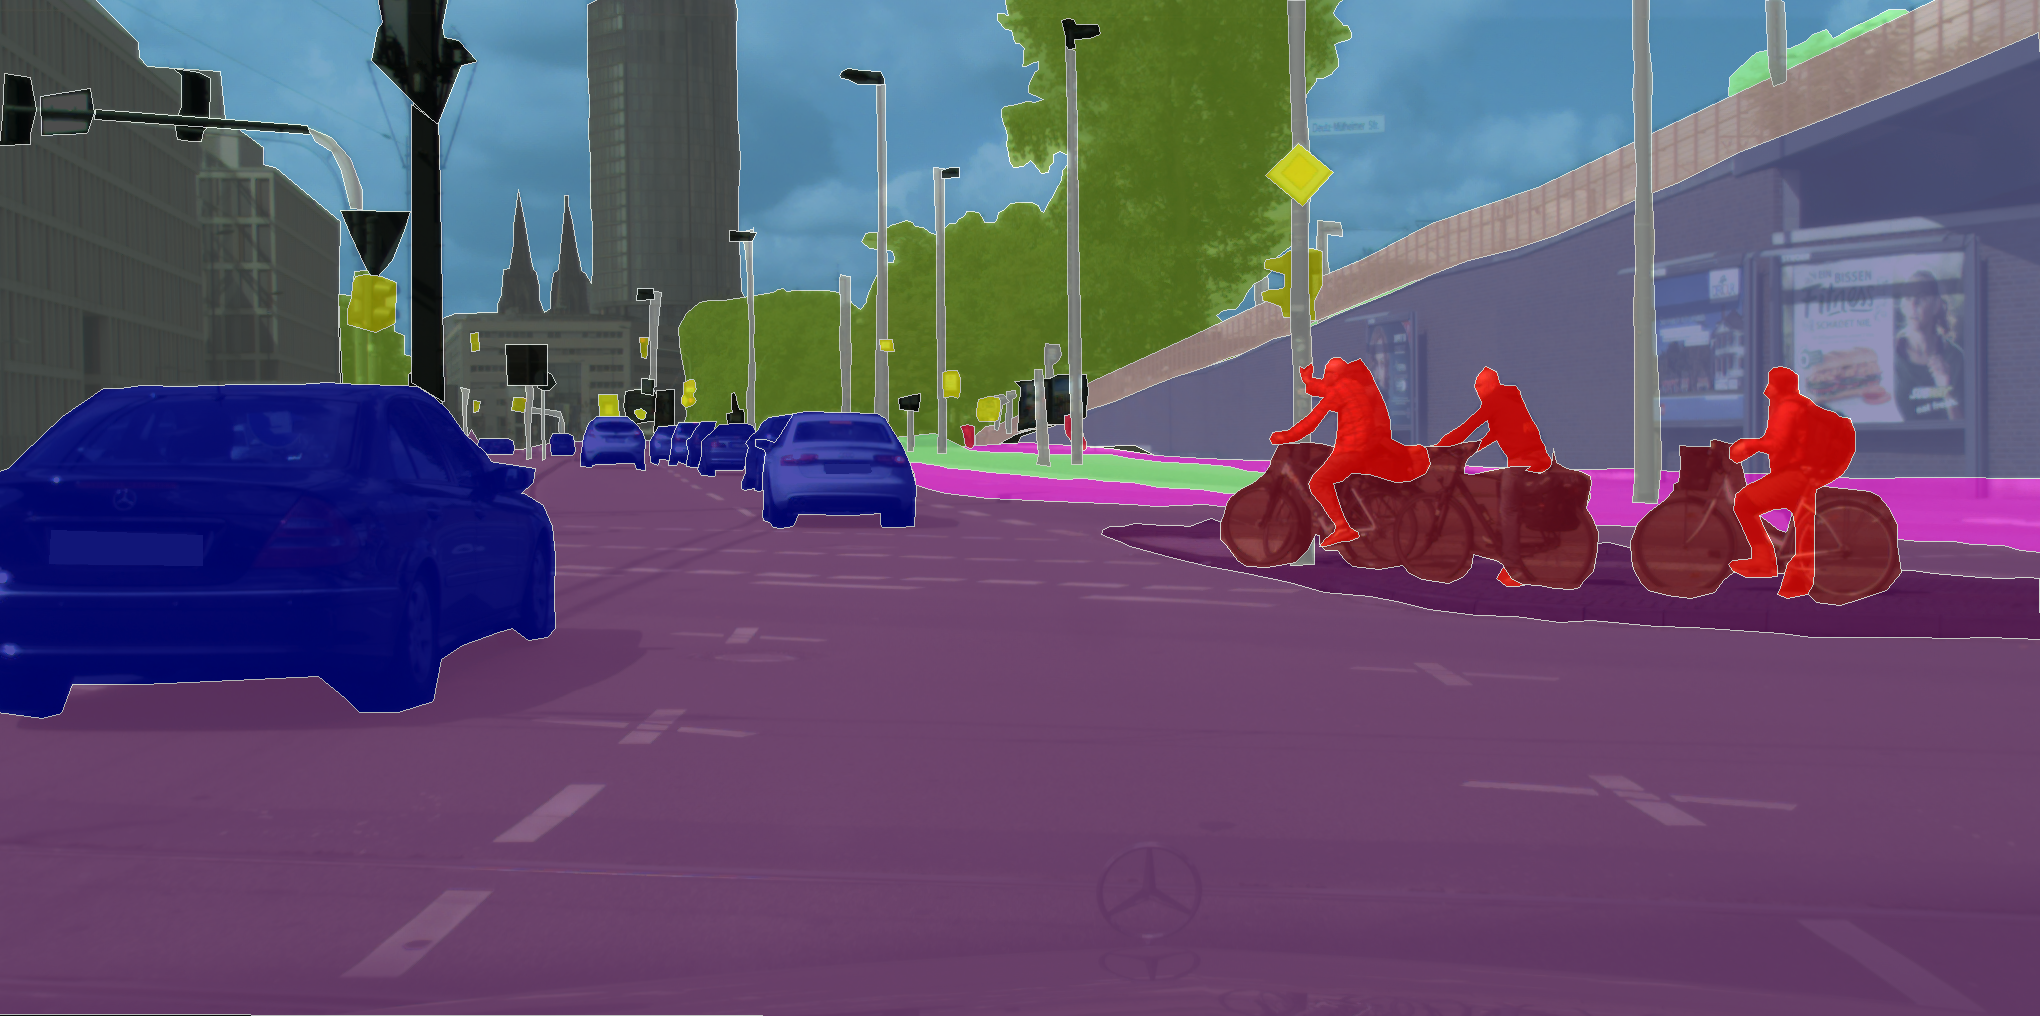
\includegraphics[width=\textwidth,keepaspectratio]{koeln00.png}
			\caption{Beispiel: CityScapes Dataset\cite{Cordts_2016_CVPR}}
		\end{figure}
	\end{column}
\end{columns}
\end{myframe}

\begin{myframe}[Motivation: (Fehlende) Ground Truths]
Ground Truth nicht immer vorhanden: Beispiel Marsoberfläche
\begin{itemize}
	\item Zu großer Datensatz
	\item Notwendigkeit von Experten
	\item[$\Rightarrow$] Manuelle Erstellung nicht kostengünstig oder zeiteffizient möglich
\end{itemize}
\medskip
Lösungsansatz:
\begin{itemize}
	\item Anfangs zufällige Klassifizierung durch Segmentierungsalgorithmus weiter optimieren
\end{itemize}
\end{myframe}

\section{Verwandte Arbeiten}

\begin{myframe}[Verwandte Arbeiten: Segmentierung nach Kanezaki\cite{kanezaki2018_unsupervised_segmentation}]
Asako Kanezaki; Unsupervised Image Segmentation by Backpropagation\cite{kanezaki2018_unsupervised_segmentation}:
\begin{columns}
	\begin{column}{.5\textwidth}
		\begin{itemize}
			\item Unüberwachtes Lernen der Segmentierung
			\item Anfangs zufällige Ergebnisse werden mit Clusteringalgorithmus vereint
			\item Zielfunktion: Softmax-Loss zwischen Ergebnis des NN und des optimierten Ergebnisses
			\item NN wird auf diese Zielfunktion hin optimiert (Backpropagation)
		\end{itemize}
	\end{column}
	\begin{column}{.5\textwidth}
		\begin{figure}
			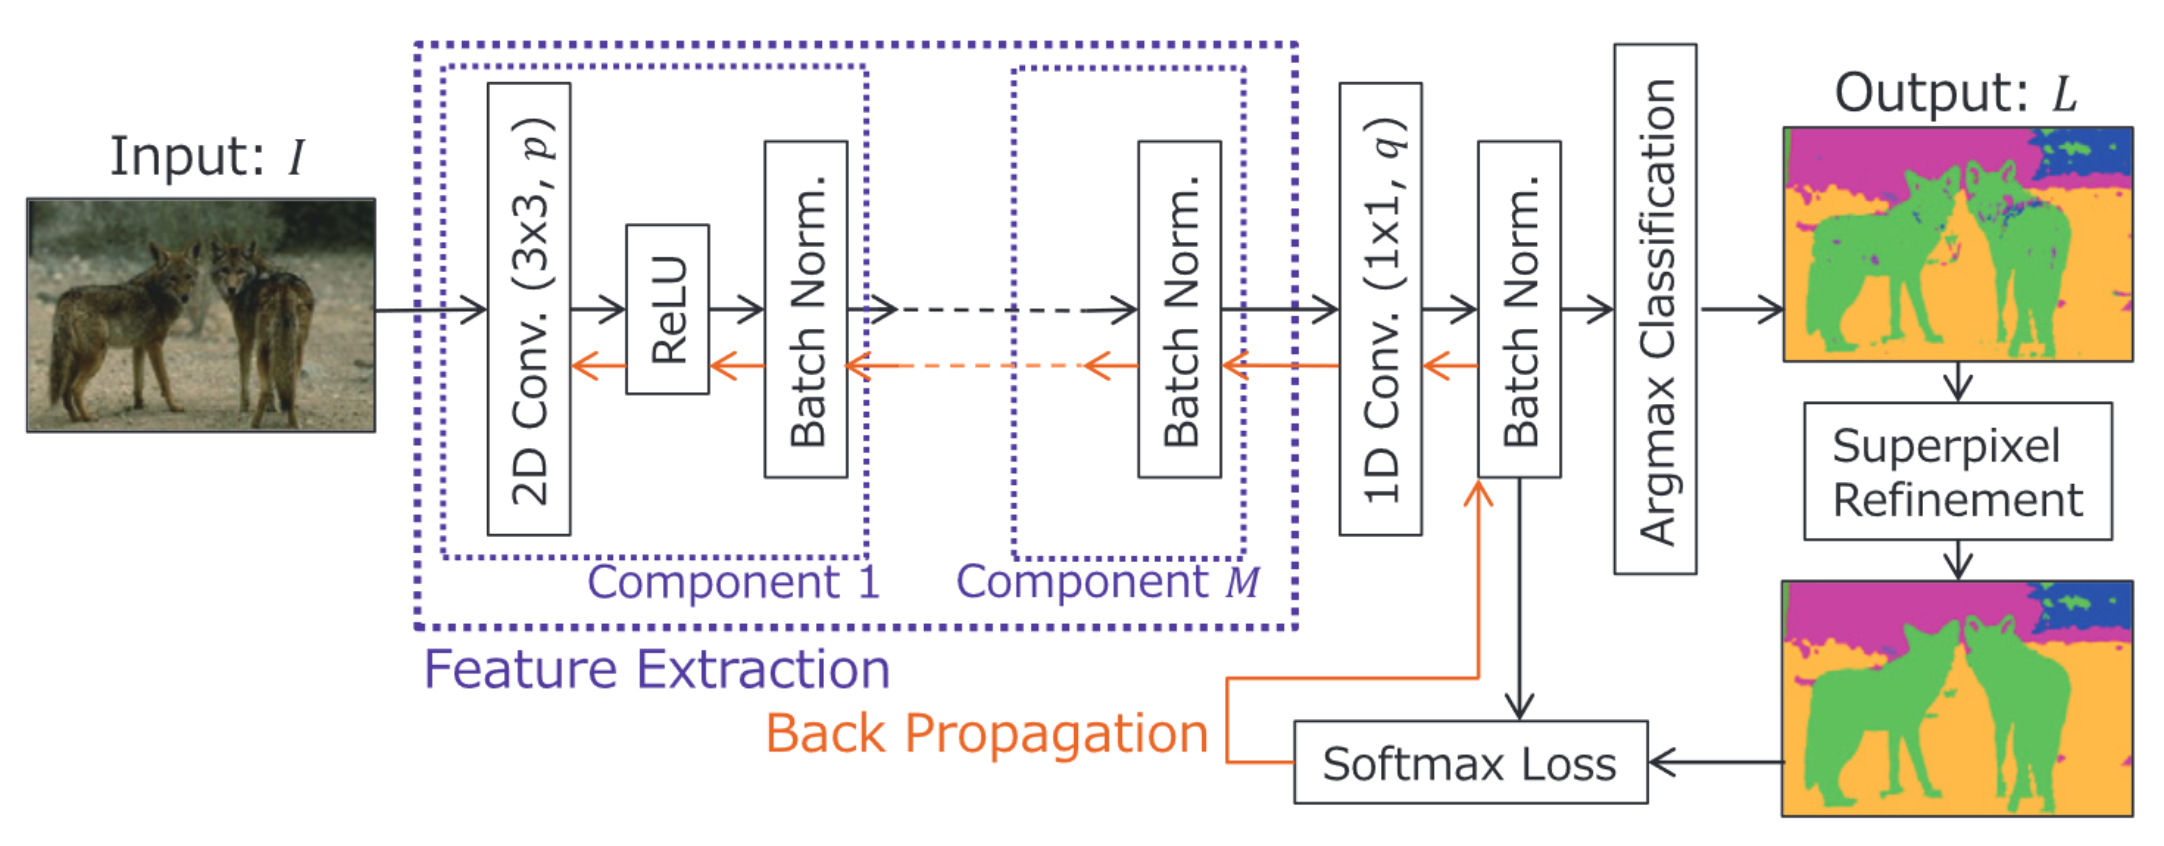
\includegraphics[width=\textwidth,keepaspectratio]{kanezaki.png}
			\caption{Vorgehensweise nach Kanezaki\cite{kanezaki2018_unsupervised_segmentation}}
		\end{figure}
	\end{column}
\end{columns}
\end{myframe}

\begin{myframe}[Verwandte Arbeiten: \textit{Crater Detection via CNNs}\cite{2016arXiv160100978C}]
	
\end{myframe}

\section{Vorgehensweise}

\section{Referenzen}

\begin{myframe}[Referenzen]
	\bibliographystyle{abbrv}
	\bibliography{presentation}
\end{myframe}

	
\end{document}